%!TEX program = xelatex
% 完整编译方法 1 pdflatex -> bibtex -> pdflatex -> pdflatex
% 完整编译方法 2: xelatex -> bibtex -> xelatex -> xelatex
\documentclass[lang=cn,11pt,a4paper,cite=number]{elegantpaper}

\title{动态规划与人工神经网络在强化学习问题中的应用}
\author{{周韧哲} \quad {zhourz@smail.nju.edu.cn}}

\institute{南京大学 \; 人工智能学院}
\date{}


\begin{document}

\maketitle

\begin{abstract}
$\text{ }\quad$强化学习(Reinforcement Learning)属于人工智能的一个子领域,其本质是对一类序列决策问题进行数学建模并解决。和有监督学习或无监督学习等其他机器学习方法相比,强化学习更加注重在与环境的交互中获得的奖励信号,并将其作为目标进行学习。强化学习算法通过试错(trial and error)来学习如何决策,环境对其决策的积极反馈就是奖励,而消极反馈则是对其犯错的惩罚。强化学习最早来源于最优控制问题,Richard Bellman等人尝试分析动态系统的状态函数和值函数,并通过动态规划来解决此类问题。后来研究者将强化学习拓展到连续空间,通过设计人工神经网络来解决强化学习问题。本文将会介绍动态规划和神经网络在强化学习问题中的应用,并给出一些重要算法的表述,最后介绍在强化学习领域的最新进展和一些自己的思考。
\keywords{强化学习 \; 马尔科夫决策过程 \; 动态规划 \; 神经网络}
\end{abstract}

\section{介绍}
强化学习通常将一类序列决策问题用马尔科夫决策过程(Markov Decision Process)建模。这一类序列决策问题包括有:令一个机器人学会走路、玩电子游戏、下围棋、学会驾驶汽车等等,即智能体在时间$t$内给出符合当前环境下的一个动作。马尔科夫决策过程最常用于建模序列决策问题,其描述如下:首先我们有一个进行进行学习和决策的智能体,智能体之外和其交互的称之为环境,智能体能感知到其所处的环境的状态,并给出一个相应的动作,环境对这些动作做出响应,转移到另一个状态,并给出一个奖励。其形式化表述为:
\begin{definition}
	一个马尔科夫决策过程是一个五元组$(\mathcal{S},\mathcal{A},\mathcal{P},\mathcal{R},\gamma)$,其中$\mathcal{S}$是状态空间,$\mathcal{A}$是动作空间。$\mathcal{P}$是状态转移概率函数,也成为动力函数,描述了在状态$s$采取动作$a$转移到的下一个状态为$s'$的概率。动力函数满足马尔科夫性,下一个状态只与当前状态与采取的动作有关,即$\mathcal{P}_{ss'}^a=\mathbb{P}[S_{t+1}=s'|S_t=s,A_t=a]$。$\gamma$是衰减因子,$\mathcal{R}$是奖励函数,$\mathcal{R}(s,a,s')$即代表在状态$s$采取动作$a$转移到了状态$s'$后所能获得的奖励。
\end{definition}
在给定一个初始状态后,智能体在每个离散时间$t=0,1,2,\cdots$都采取动作与环境发生交互并获得奖励,这称之为一个交互轨迹:$\tau=(s_0,a_0,r_0,s_{1},a_{1},r_{1},\cdots)$。智能体从交互中学习策略$\pi(a|s)$,其意义为在状态s时选择动作a的概率。在任意离散时刻$t$,智能体的目标是最大化期望累积奖赏$G_t\doteq\sum_{i=0}^T\gamma^{i} r_{t+i}$。即智能体并非要最大化当前的奖励,它会考虑长期的回报,并且通过衰减因子$\gamma$体现了离现在越远的奖励权重越低。一个典型的马尔科夫决策过程框架如图\ref{fig:fig1}所示:
\begin{figure}
	\centering
	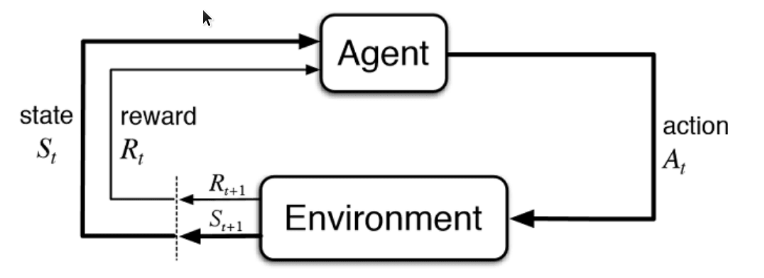
\includegraphics[width=0.8\linewidth]{figure/fig1}
	\caption{典型MDP框架\cite{rl}}
	\label{fig:fig1}
\end{figure}

给定了这样一个马尔科夫决策过程,我们还需要定义策略的价值函数。
\begin{definition}
	策略$\pi$下状态$s$的价值函数为$$v_\pi(s)\doteq\mathbb{E}_{\pi}[G_t|S_t=s]$$其意义为在状态$s$下智能体服从策略$\pi$进行决策的期望回报值,称之为状态值函数。
\end{definition}
\begin{definition}
	策略$\pi$下状态动作对$(s,a)$的价值函数为$$q_\pi(s,a)\doteq\mathbb{E}_{\pi}[G_t|S_t=s,A_t=a]$$其意义为在状态$s$下采取动作$a$后,智能体在$\pi$下的所有决策的期望回报值,称之为动作值函数。
\end{definition}
直观来看,状态值函数评估了当前状态好不好,动作值函数评估了在当前状态下采取的一个动作好不好。状态值函数与动作值函数存在关系,由定义容易知道$v_\pi(s)=\mathbb{E}_{a\sim\pi(a|s)}[q_\pi(s,a)]$,$q_{\pi}(s,a)=\mathbb{E}_{s'\sim p(s'|s,a)}[r+\gamma v_{\pi}(s')]$。事实上,这两者的关系可由图\ref{fig:fig2}形象说明。空心结点代表状态,实心结点代表动作。
\begin{figure}
	\centering
	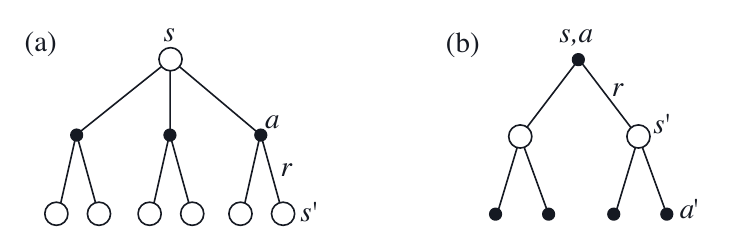
\includegraphics[width=0.8\linewidth]{figure/fig2}
	\caption{$v_\pi(s)$和$q_\pi(s,a)$的回溯图\cite{rl}}
	\label{fig:fig2}
\end{figure}


智能体的目标就是寻找一个最优策略,使得这个策略在所有可能策略集合中的期望回报最大,即最大化$\mathbb{E}_{\tau\sim\pi}[G(\tau)]=\mathbb{E}_{\tau\sim\pi}[\sum_{t=0}^{\infty}\gamma^tr_t]$。接下来我将介绍解决马尔科夫决策过程的一些方法。
\section{动态规划解决MDP问题}
动态规划是解决一类数学问题的通用方法,通过将复杂问题分解为更为简单的子问题来求解复杂问题,因此需要这一类数学问题具有重叠子问题和最优子结构。对于离散空间中的马尔科夫决策过程,Bellman给出了其递归分解,在强化学习中称之为Bellman方程。事实上,动态规划最早便是由Bellman提出的。

对于状态值函数和动作值函数,有如下Bellman方程:$$v_{\pi}(s,a)=\sum_{a}\pi(a|s)\sum_{s',r}p(s',r|s,a)(r+\gamma v_\pi(s'))$$$$q_{\pi}(s,a)=\sum_{s',r}p(s',r|s,a)(r+\gamma\sum_{a'} q_\pi(s',a'))$$

事实上,最优状态值函数$v_*(s)\doteq\max_\pi v_\pi(s)$与最优动作值函数$q_*(s,a)\doteq \max_\pi q_\pi(s,a)$也满足以上方程,称之为由Bellman最优方程。给出迭代方程后,我们就可以用动态规划来求解马尔科夫决策过程,通过近似逼近价值函数,得到最优决策。其算法主要包括策略评估、策略改进和策略迭代\cite{rl}。
\subsection{策略评估}
策略评估算法是计算一个策略的状态值函数的算法,其思想就是动态规划,首先初始化该策略下的状态值函数,然后通过Bellman方程来更新状态值函数,直到满足符合条件的误差精度即可。在每一个循环中,我们都对所有的状态基于上一次迭代的值来同时更新当前迭代的值函数。一旦当前循环中的值函数与上一次循环的值函数的最大差距小于某个给定的常数时,算法停止迭代。事实上,只要$\gamma<1$,该算法一定能收敛,即准确评估了当前策略的价值。
\subsection{策略改进}
我们评估策略的目的是为了改进策略,寻求一个价值更好的策略。因此,在给定任意一个策略的价值后,我们想对该策略作出改进,使其更优。贪心策略$\pi'$满足$$\pi'(s)=\arg\max_a q_\pi(s,a)=\arg\max_a\sum_{s',r}p(s',r|s,a)[r+\gamma v_\pi(s')]$$

事实上,这样构造出来的策略满足策略改进定理\cite{rl},即新策略一定不比原策略差。这称之为策略改进。
\subsection{策略迭代}
一旦对作出了改进后,我们可以重新评估新策略的价值,再接着对新策略作出改进。如此以来,策略迭代就能不断搜索得到更优策略直到收敛。策略迭代算法描述如图\ref{fig:fig3}所示。事实上,策略迭代可以视作策略评估和策略改进的竞争与合作,两个过程相互作用会使得其收敛到最优价值函数与最优策略。
\begin{figure}
	\centering
	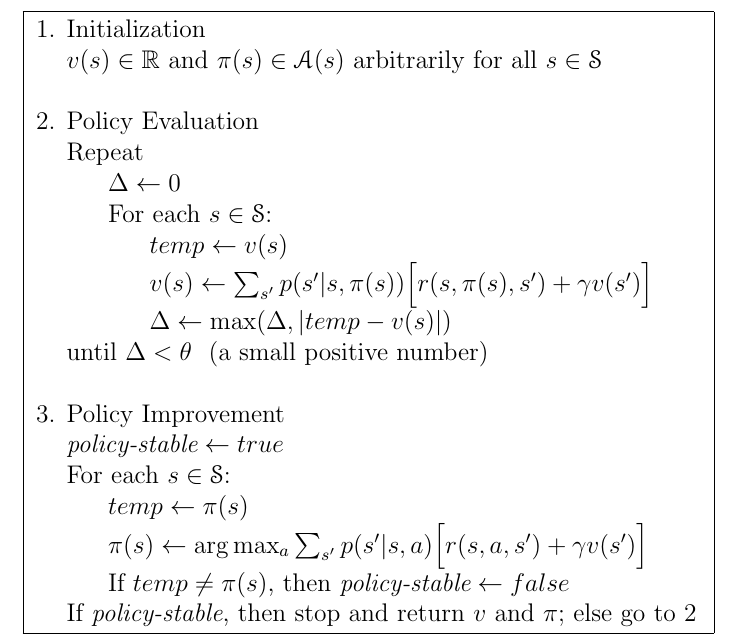
\includegraphics[width=0.83\linewidth]{figure/fig3}
	\caption{策略迭代算法\cite{rl}}
	\label{fig:fig3}
\end{figure}

动态规划适合解决离散空间的马尔科夫决策过程,且由于其需要提前知道状态转移分布,来遍历所有状态空间,因此当状态空间维度很大时,使用动态规划会难以求解。然而在现实生活遇到的问题中,状态空间和动作空间往往是高维的连续空间,因此,研究者们提出了许多方法来解决高维连续马尔科夫决策过程,比如启发式地在策略空间中搜索最优策略,使用遗传算法学习最优策略等等。目前比较成功的有估计价值函数和寻找最优策略的时序差分学习,其包括了Q学习,Sarsa和蒙特卡洛方法等等一系列算法及其变种。它们不需要提前知道环境状态转移的具体分布,而是从与环境交互得到的样本序列来进行学习,即通过智能体的“记忆”来学习,因此容易运用到高维场景中。

2012年,Hinton和Alex在国际ImageNet图像分类竞赛中使用深度卷积神经网络以远超第二名的成绩获得冠军,自此以后,深度学习飞速发展。同样地,强化学习中也引入了人工神经网络,并取得了巨大的进展。下面我将介绍神经网络在强化学习中的运用,使用人工神经网络来解决高维连续MDP问题。

\section{人工神经网络解决MDP问题}
\subsection{DQN}
\begin{figure}
	\centering
	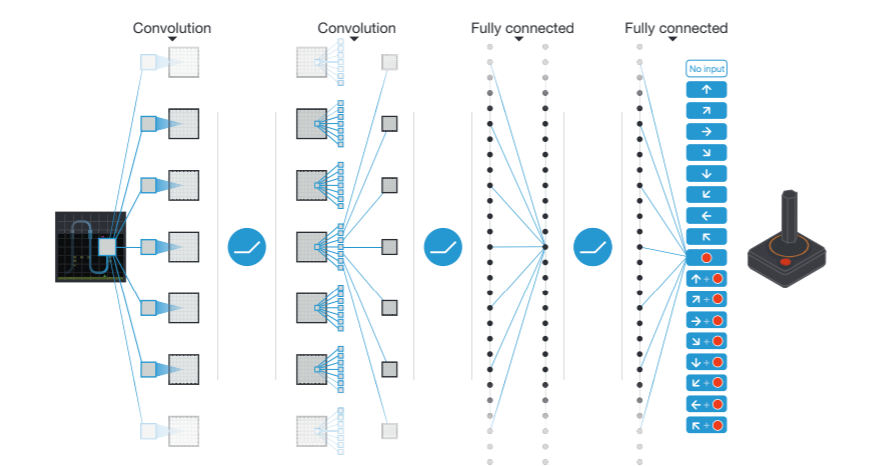
\includegraphics[width=1\linewidth]{figure/fig5}
	\caption{Atari游戏中的卷积神经网络\cite{journals/nature/MnihKSRVBGRFOPB15}}
	\label{fig:fig5}
\end{figure}

2013年,Deepmind发表论文\cite{mnih2013playing},提出DQN算法,首次将深度神经网络运用在强化学习中,是第一个有广泛影响力的深度强化学习系统。研究人员的任务是令智能体学会玩七个Atari 2600游戏,他们将此任务建模为一个马尔科夫决策过程,并使用同一个结构的卷积神经网络来建模值函数,使用Q学习的方法进行强化学习的训练,结果在六个游戏中均表现优异,在其中三个游戏中的表现超过了人类专家的水平。这显示了将人工神经网络运用在强化学习中的巨大能量。2015年,Deepmind再次发表论文\cite{journals/nature/MnihKSRVBGRFOPB15},将DQN算法改进后运用与Atari 2600游戏,在43个Atari 2600电动游戏上的性能超过了之前最好的强化学习算法,在29个Atari 2600电动游戏上达到了人类玩家的水平(75\%的得分)。

DQN(Deep Q-Learning Net)使用了卷积神经网络来表示动作值函数$Q(s,a)$,我们称之为Q网络。网络把游戏中连续的4帧图片作为状态输入,输出在该状态下各个动作的值。其架构如图\ref{fig:fig5}所示。智能体通过与游戏环境交互获得轨迹,将轨迹中的每一个样本$(s_t,a_t,s_{t+1},r_t)$都存储在经验回放池(Replay Buffer)中。DQN中的Q网络有两个,分为评价网络和目标网络,两者的结构都相同。评价网络用来计算Q值,每次迭代都会更新该网络的权重。目标网络作为学习的目标,不会在每次迭代都更新,而是在完成一定次数的更新后,再将评价网络的权重赋给目标网络,进而进行下一批更新,用于解决训练不稳定问题。每次更新网络时,都从经验回放池中采样一批样本,网络的损失函数是$$\mathbb{E}_{(s,a,s',r)}[(r+\gamma\max_{a'}Q_{target}(s',a')-Q_{eval}(s,a))^2]$$其中$Q_{eval}(s,a)$就相当于网络的预测值,而$r+\gamma\max_{a'} Q_{target}(s',a')$就相当于目标值,这就类似于监督学习中的样本标签与预测标签的均方误差,可以使用梯度下降方法来优化。其算法描述如图\ref{fig:fig6}所示。
\begin{figure}
	\centering
	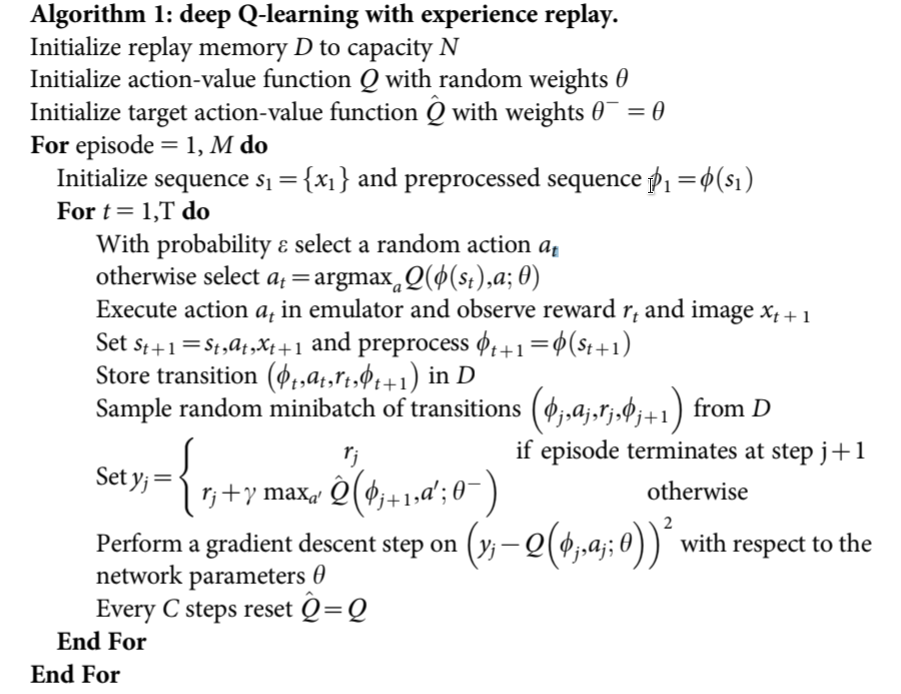
\includegraphics[width=0.9\linewidth]{figure/fig6}
	\caption{DQN伪代码\cite{journals/nature/MnihKSRVBGRFOPB15}}
	\label{fig:fig6}
\end{figure}
\subsection{策略梯度}
DQN是基于值函数近似的方法,它预测每个状态下所有动作的期望价值,且借助于神经网络的表达成功地解决了高维连续状态空间的MDP问题。但是DQN输出的策略是确定性贪心策略,即在任意状态下每次均选择期望价值最大的动作。而现实生活中很多问题的动作空间是连续空间,不同于学习选择每个行动的概率,它需要智能体学会一个随机策略,即一个关于动作的分布$\mathcal{P}(a|s)$,在连续行动空间中学习概率分布的统计量,从而对不确定性进行了建模,不同于DQN等基于价值来解决MDP问题,基于策略的强化学习方法试图直接在策略空间中优化策略函数,而非先求得环境状态或动作的价值后再根据动作价值来确定策略,通过不断计算策略期望总回报关于策略参数的梯度来更新策略参数,最终收敛于最优策略。

策略梯度方法通常用一个高斯分布来建模策略,即认为$\pi(a|s)\sim\mathcal{N}(\mu,\sigma^2)$,并且直接优化期望回报$\mathcal{J}(\theta)=\mathbb{E}_{\tau\sim\pi_\theta(a|s)}[\sum_{t=0}^{\infty}\gamma^tr_t]$。等人给出了策略梯度定理,证明了该函数的梯度$\nabla_\theta\mathcal{J}(\theta)\propto\sum_s\mu(s)\sum_a q_\pi(s,a)\nabla\pi_\theta(a|s)$。这说明了策略梯度的目标函数对策略的参数$\theta$的梯度可根据策略对其参数$\theta$的梯度求得,而和状态概率对策略的参数$\theta$的梯度无关,很大程度上简化了计算的难度,只需要通过梯度上升方法来更新策略参数,即$\theta_{new}=\theta_{old}+\alpha\nabla_\theta\mathcal{J}_\theta$。但是不同于监督学习,在策略梯度方法中学习率$\alpha$的设置是一个很大的问题,如何保证每次策略参数更新能带来策略性能的单调提升是一个难点,而且通过神经网络直接在策略空间进行策略搜索代价很高,也容易陷入局部最优解而无法取得全局最优解。

Proximal Policy Optimization(近端策略优化)是OpenAI发表的一种策略优化算法\cite{schulman2017proximal},把惩罚项设计进目标函数,使策略优化过程变得更简单有效,能够有效地优化大规模的非线性策略,如通过深度神经网络拟合的策略。PPO采用了Actor-Critic架构。Actor-Critic通过引入一种评价机制来解决MDP问题,Actor就是策略,建模了动作分布,给定一个状态,Actor会从自身的分布中给出一个动作;Critic类似于策略评估,可以看成是动作值函数$q_{\pi_\theta}(s,a)$,对Actor的动作进行评估,并且计算优势函数(给定状态$s$,某个动作$a$相对于平均而言的优势),引导Actor参数在梯度方向上走得更好。Actor根据Critic的评估来决定对参数的调整。其运行步骤如下:
\begin{enumerate}
	\item Actor和环境交互,将交互样本存储在Replay Buffer中。
	\item Critic根据Replay Buffer中的数据更新Critic参数。
	\item Actor根据Replay Buffer中的数据和Critic计算出来的优势函数更新Actor参数。
\end{enumerate}
Actor-Critic架构的流程可见图\ref{fig:fig9}。
PPO在更新Actor策略时,使用当前Replay Buffer中的数据在策略上采取最大可能的改进,同时也采用一阶方法的技巧来使新策略接近于旧策略,从而使得策略不会走得太远而意外导致性能下降。其算法描述如图\ref{fig:fig8}所示。
\begin{figure}
	\centering
	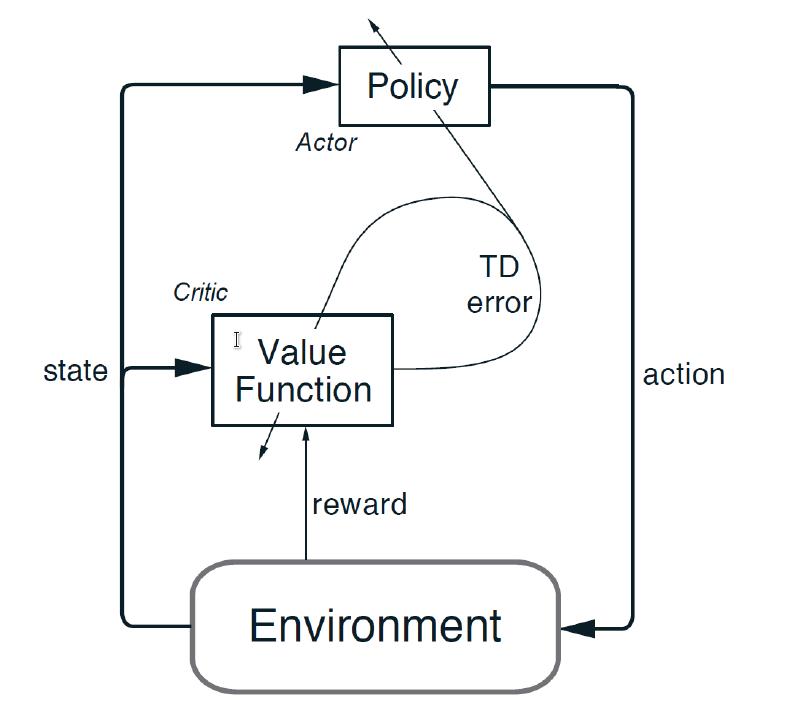
\includegraphics[width=0.6\linewidth]{figure/fig9}
	\caption{Actor-Critic架构}
	\label{fig:fig9}
\end{figure}

\begin{figure}
	\centering
	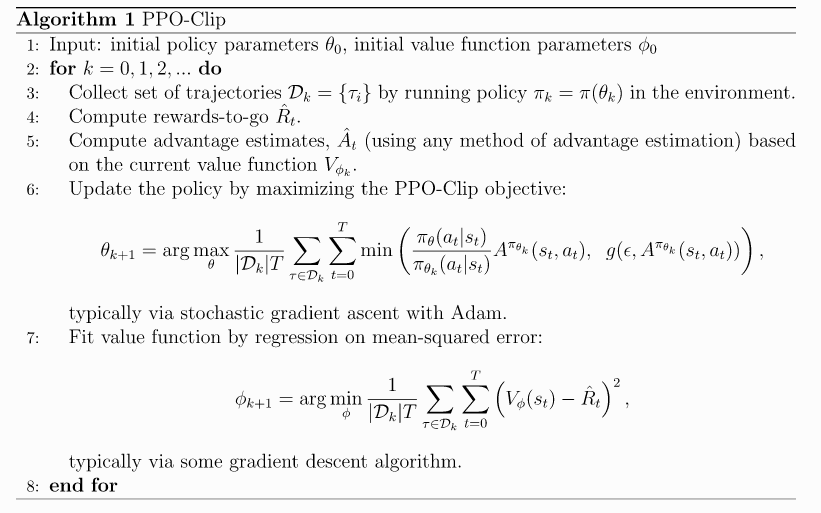
\includegraphics[width=1\linewidth]{figure/fig8}
	\caption{PPO伪代码\cite{schulman2017proximal}}
	\label{fig:fig8}
\end{figure}


\section{前沿}
DQN和PPO一个属于基于价值函数方法,一个属于策略梯度方法,但都将人工神经网络运用于强化学习问题解决MDP问题从而取得了巨大的成功。目前的深度强化学习领域十分火热,前沿研究主要包括基于模型(model-based)的强化学习、模仿学习(imitation learning)、离线(offline)强化学习等等。这里我将介绍几个强化学习前沿领域。
\subsection{生成对抗模仿学习}
模仿学习通过从专家样本中学习来决策,没有环境的奖赏反馈信号,并假设专家样本由某个最优策略采集而来,智能体要从这有限的专家样本中学出一个较好的策略。生成对抗模仿学习(Generative Adversarial Imitation Learning,GAIL)是基于生成对抗网络的模仿学习,其最早由HO等研究者\cite{ho2016generative}提出。GAIL结合了GAN\cite{goodfellow2014generative}的思想,从博弈论角度建模这个问题。在GAN中,生成器被训练为生成接近与真实图片的生成图片,而判别器则被训练为尽可能地分辨真实图片和生成图片,两者互相博弈对抗,生成器在判别器提供的信号下会渐渐生成十分接近真实图片的生成图片。

在GAIL中,生成器和环境交互产生一系列生成轨迹样本$(s,a)$,而判别器则被训练为尽可能地分辨专家样本和生成样本。判别器用一个神经网络$D(s,a)$表示,输出一个$[0,1]$区间的实数值,可以看作是判别器认为输入样本为专家样本的概率。生成器可以看作是一个策略,用Actor-Critic架构表示,根据状态$s$输出一个动作$a$,而这一个样本对应的奖赏则是判别器的输出$D(s,a)$。生成器在判别器提供的奖励信号下,不断生成接近于专家样本的数据,不断靠近专家策略的分布,判别器与生成器互相对抗,从而学得一个表现优异的策略。

AIRL\cite{fu2018learning}是另一种生成对抗模仿学习方法,因为GAIL并没有显式地学得一个奖赏函数,AIRL提出了另一种判别器的神经网络架构$D=\frac{\exp(f(s,a,s'))}{\exp(f(s,a,s'))+\pi(a|s)}$,其中$f(s,a,s')=R(s,a)+\gamma V(s')-V(s)$,由两个神经网络$R(s,a)$和 $V(s)$表示,可以显式地表达出奖励函数的形式,从而可以进行迁移学习。

后来的研究者也从GAIL和AIRL中进行改进,提出了一些更优异鲁棒的生成对抗模仿学习方法,如CGAIL\cite{9266753}、VAE-GAIL\cite{NIPS2017_044a23ca}、Info-GAIL\cite{sharma2019directedinfo}等。
\subsection{基于模型的强化学习}
一般的强化学习都需要智能体与环境交互生成数据,这称之为免模型学习。而基于模型的强化学习则认为环境不易得到或者与环境交互的成本很高,所以需要先对环境建模,学得一个能够模拟真实环境的模型$T(s'|s,a)$,即给定状态$s$和动作$a$,返回下一个状态$s'$。然后令策略与学得的模型交互,运用通用的强化学习方法来优化策略。

最简单的基于模型的强化学习使用监督学习来学习环境模型,即在一批交互数据$(s,a,s')$中把$(s,a)$当成输入,$s'$当成标签进行监督学习,如Marc等研究者\cite{j}将模型建模为一个高斯分布,使用平方指数核函数误差来学习模型。但是这样需要很大的样本集,且模型的compounding error(复合误差)被南京大学许天、俞扬等研究者证明是随着目标函数值的差异以二次方的速度增长的\cite{xu2020error}。为了降低误差,Michael等研究者\cite{janner2019trust}使用多个模型做集成学习,在一百万条数据集上取得了不错的效果。

不同于上述的监督学习只考虑one-step error:$\min_s\mathbb{E}[(s-s_{label})^2]$,Wu等研究者\cite{wu2020model}从n-step estimate(多步估计)中学习模型$T(s'|s,a)$,考虑将模仿学习应用在模型学习中。给出某个策略下的真实交互样本集,把策略和模型的角色互换,当策略给定时,策略与模型交互产生轨迹。这里的生成器就是需要学习的环境模型$T$,使用WGAN\cite{arjovsky2017wasserstein}来分辨真实轨迹和生成轨迹并提供奖励信号,从而通过生成对抗模仿学习学出了环境模型。南京大学许天、俞扬等研究者证明了使用模仿学习学得的模型的compounding error是随着目标函数值的差异以一次方的速度增长的\cite{xu2020error}。
\section{总结}
本文介绍了动态规划和神经网络在强化学习问题中的应用,并给出一些重要算法的表述。强化学习的基础是马尔科夫决策过程,通过将序列决策过程数学建模成为马尔科夫决策过程,提炼出了序列决策过程的本质。动态规划是解决低维离散空间的马尔科夫决策过程的有效算法,而当其拓展到高维连续空间时,人工神经网络建模的深度强化学习便是解决这一类问题的有效途径。自2013年以来,强化学习在不同领域取得了巨大的进展,尤其是在棋类博弈、多智能体合作游戏、机器人控制等领域。不少研究人员认为结合了深度学习的表示能力与强化学习的推理能力的深度强化学习会是通往通用人工智能的途径。但是,深度强化学习中的可复现性差、样本利用率低、难以设计好的奖励函数、难以平衡探索和利用、灾难性的不稳定性等问题依然困扰着诸多研究人员。我认为其解决方法在于回归到强化学习的数学模型本质,从数学上找到一些解决上述难题的方法。而且我认为不必对深度强化学习过于乐观,我们不应该对一个深度学习任务强行将其强化学习化,而是应该针对一些天然适合强化学习处理的任务,尝试通过引入深度学习来提升现有方法的能力,解决模拟器与真实世界环境间的差异,从而可以发挥强化学习的强大威力。


\bibliography{reference}

\end{document}
